%TEX root = ../dissertation.tex

\chapter{Implementation}
\label{chapter:implementation}

For our Pulsarcast implementation, we decided to take advantage of the
\emph{libp2p} ecosystem as it solves a lot of the underlying issues of building
a peer to peer system, not specific to our pub-sub scenario. This includes
dealing with connection multiplexing, \acrshort{nat} traversal, discovery
mechanisms and others.  All of which libp2p, a community-focused project with
implementations in multiple languages already solves. We can also take
advantage of the utility modules it has and the advantage of having an already
working implementation of the Kadmelia \acrshort{dht}. Our focus is then to
build a module, implementing the Pulsarcast specification that clients and apps
can take advantage of. Section \ref{pulsarcast-javascript-module} provides a
detailed description of it.

Besides our module, we also needed to find a suitable way to test our system as
a whole. Given our specific needs, we opted to build a custom testbed, detailed
in Section \ref{sec:testbed} and the basis of the evaluation detailed in Chapter
\ref{chapter:evaluation}. 

\section{Pulscarcast Javascript module}\label{pulsarcast-javascript-module}

We chose to implement our Pulsarcast module in Javascript. As we covered in our
related work, Javascript is ubiquitous, running in browsers, servers and many
different kinds of devices and architectures. Through it, we can run our
Pulscarcast nodes in a multitude of systems and most importantly, direct its
usage for the World Wide Web. Plus, libp2p has a Javascript implementation
focused on cross-compatibility between server and browser. This is not to say
that in the future we will not have other implementations in different
languages, that is, in fact, one of the reasons for the clear separation
between the Pulcarcast specification and its actual implementation.  However,
we had to choose, and in our view, Javascript is the clear winner. It is worth
noting that, much like the work we built on top of, this module is open
source~\footnote{\url{https://github.com/JGAntunes/js-pulsarcast}}.

\subsection{Dependencies}\label{subsec:dependencies}

Figure \ref{fig:pulsarcast-in-libp2p} gives us an overview of how our module
fits in the libp2p ecosystem. libp2p defines interfaces responsible for routing
content (peer routing), discovering other peers in the network (peer
discovery), network transports and leveraging multiple network connections
(switch). These all come bundled in the libp2p javascript
module~\footnote{\url{https://github.com/libp2p/js-libp2}} which we use in
Pulsarcast. Besides the main libp2p module we also use some other utility
modules such as the \acrshort{cid}
module~\footnote{\url{https://github.com/multiformats/js-cid}} and the Peer-id
module~\footnote{\url{https://github.com/libp2p/js-peer-id}}, both designed to reason
with content identifiers (peer identifiers are also content identifiers). 

\begin{figure}[hb!]
  \centering
  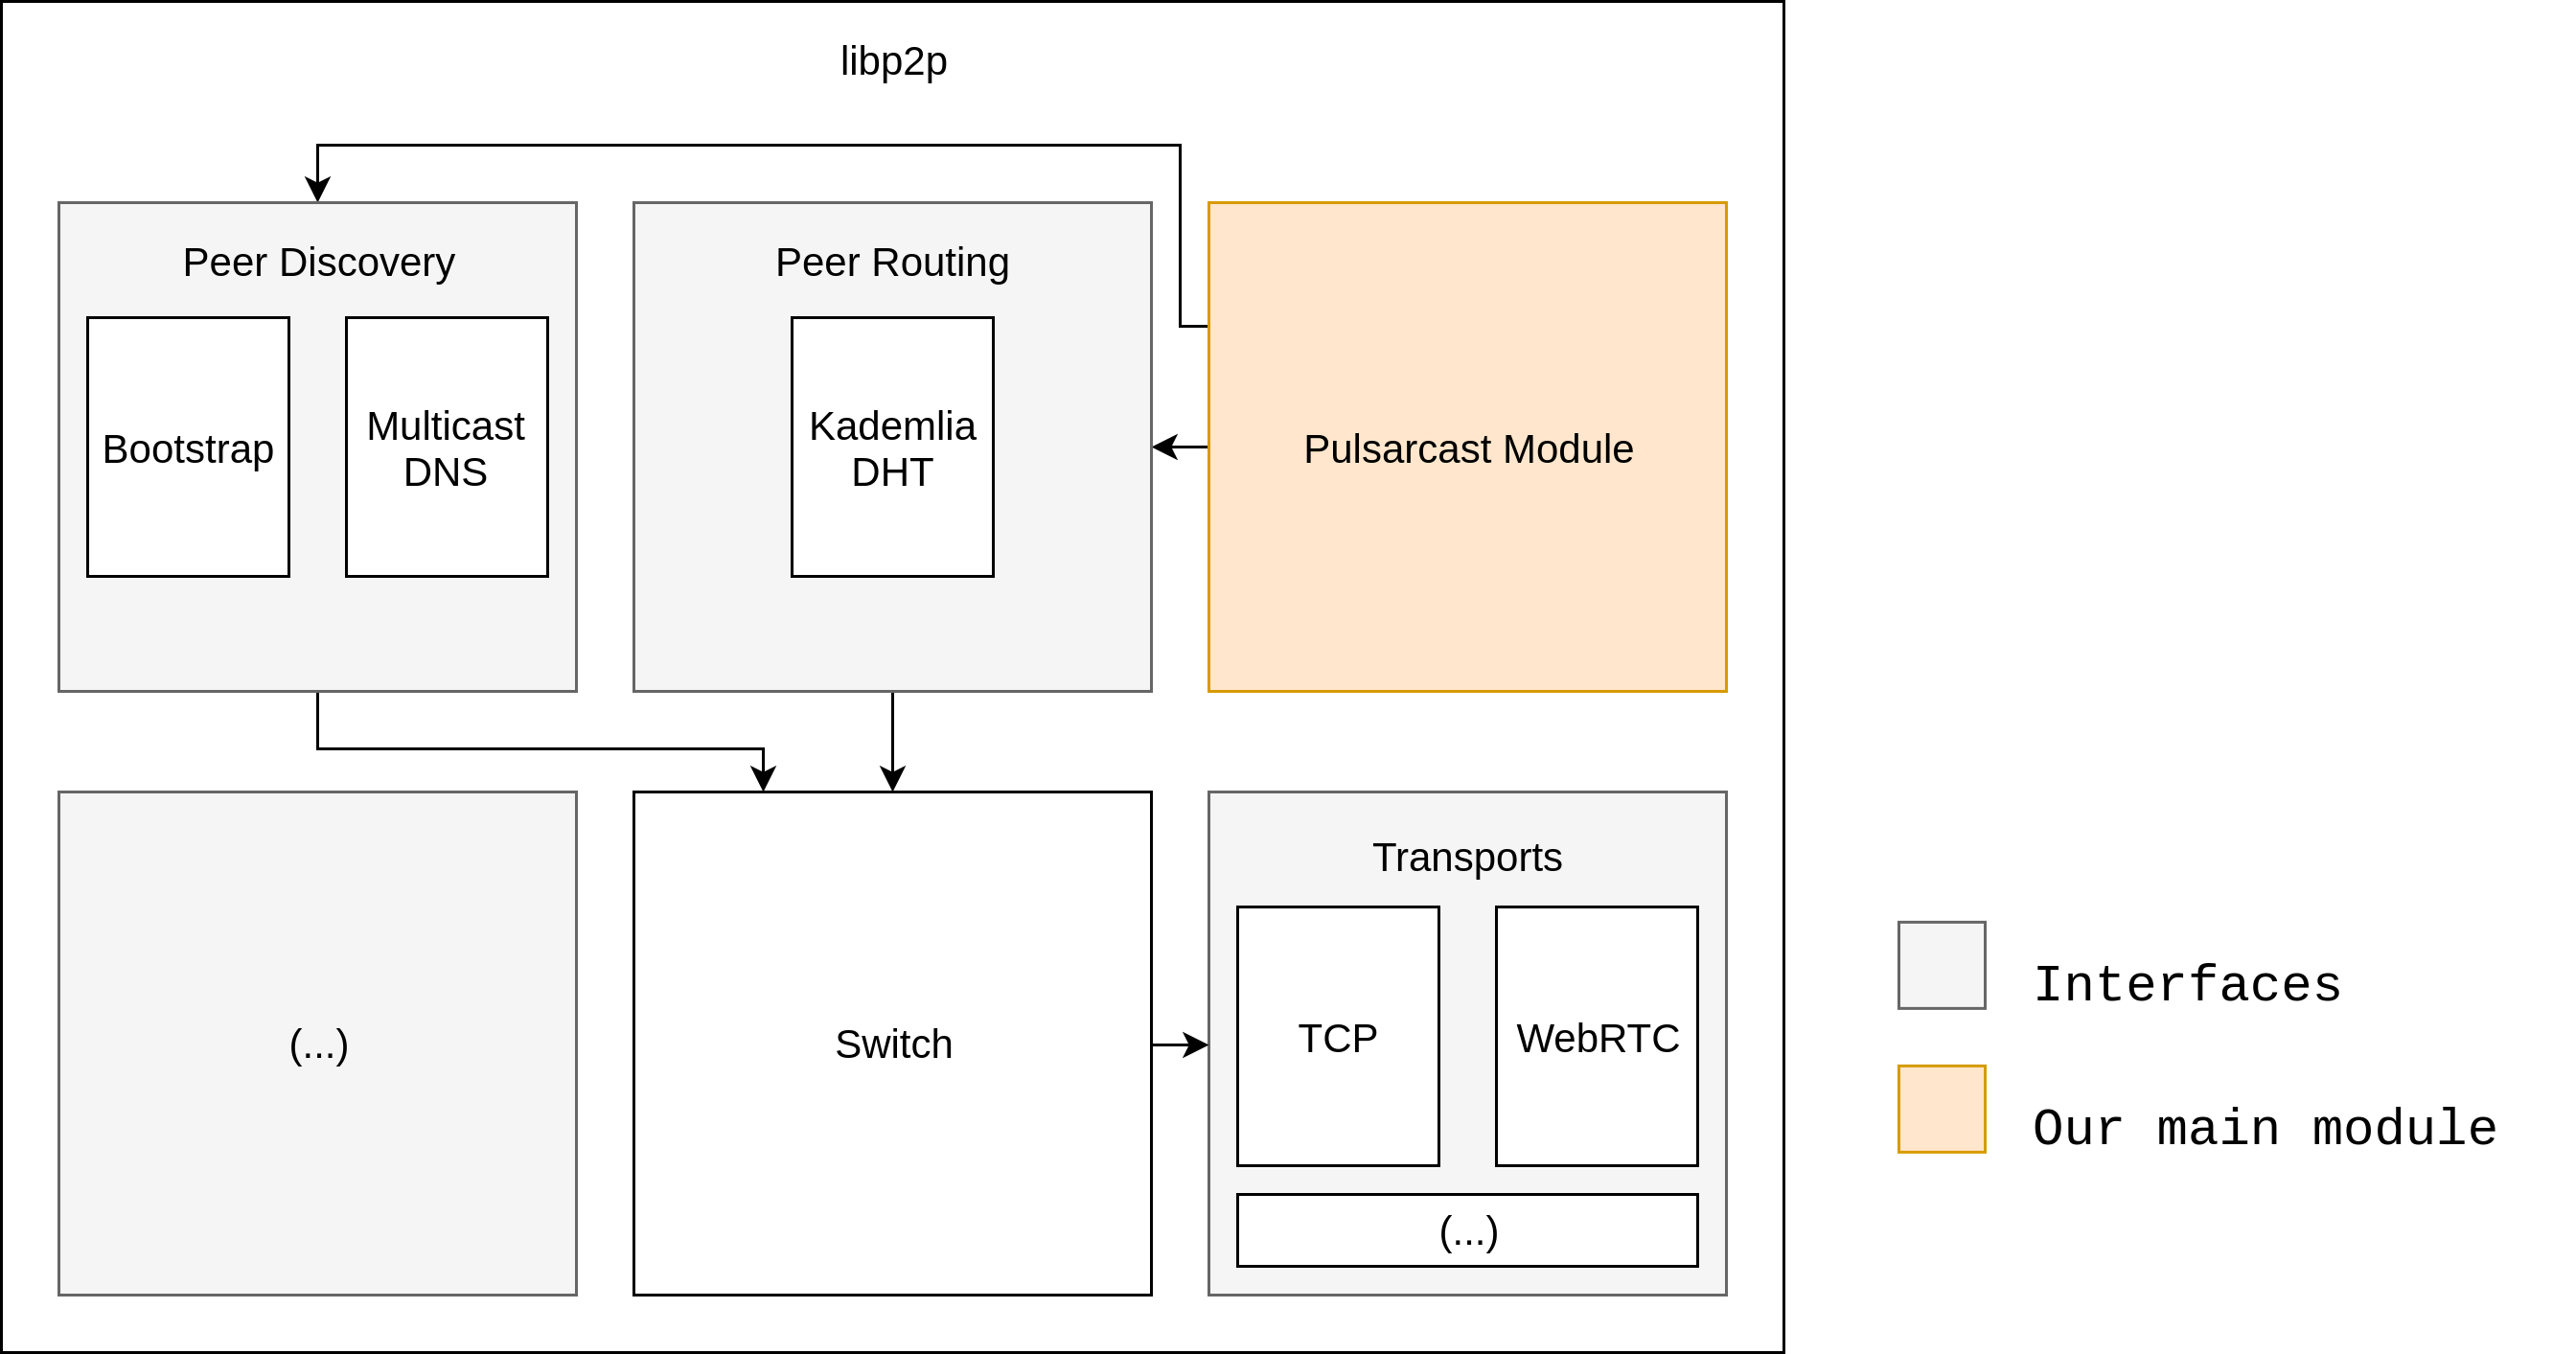
\includegraphics[width=0.95\textwidth]{img/pulsarcast-in-libp2p.png}
  \caption{Our Pulsarcast module in the libp2p ecosystem}
  \label{fig:pulsarcast-in-libp2p}
\end{figure}

Other than the libp2p dependencies, we have used other open source community
modules. Listing \ref{dependencies} shows our dependency list, pulled from our \emph{package.json} (our module manifest). We have used a couple of helpers
for handling data streams~\footnote{\url{https://github.com/pull-stream/pull-stream}}
as well as a library to help us with the asynchronous control
flow~\footnote{\url{https://github.com/caolan/async}}. To help us with protocol
buffers, we use protons~\footnote{\url{https://github.com/ipfs/protons}} and finally,
joi~\footnote{\url{https://github.com/hapijs/joi}} is our validation library of
choice.

% \noindent\begin{minipage}{\textwidth}
% \vspace{8pt}
\begin{lstlisting}[language=JSON, float, caption={Pulsarcast module dependency list},label={dependencies}]
{
	...
	"dependencies": {
		"async": "^2.6.1",
		"bs58": "^4.0.1",
		"cids": "^0.5.5",
		"debug": "^3.1.0",
		"ipld-dag-cbor": "^0.13.0",
		"joi": "^13.4.0",
		"joi-browser": "^13.4.0",
		"peer-id": "^0.12.2",
		"peer-info": "^0.14.1",
		"protons": "^1.0.1",
		"pull-length-prefixed": "^1.3.1",
		"pull-stream": "^3.6.9"
	},
	...
}
\end{lstlisting}
% \vspace{8pt}
% \end{minipage}

\subsection{Code Organisation}\label{subsec:code-organisation}

When it comes to code organisation, and despite not existing a clear standard
for modules in Javascript, we follow what is most generally conceived as best
practices. Listing \ref{file-tree} gives us an overview of the file structure
of our project. 

Our \emph{src} (source) directory has all the components that constitute our
Pulsarcast node. \emph{src/index.js} holds our top-level class, Pulsarcast,
that is exported and listed as the main component to import when applications
\emph{require} our module. We have split internal components into folders
according to its functionality. The classes for our event and topic
descriptors, as well as its trees, are under the \emph{dag} directory. The
\emph{messages} directory keeps all the important pieces of functionality
relative to our \acrshort{rpc} messages, including its Protocol buffers,
validators and marshalling logic. Our \acrshort{rpc} handlers, containing
Pulsarcast's core algorithms and logic, are kept under \emph{rpc}. Finally, on
the root of our source directory, we keep our default node configuration, our
peer class and an \emph{utils} directory, where we store a series of utility
functions used across our codebase.

Apart from our source directory, we have a series of unit and integration
tests, currently kept under \emph{test}. These tests exercise the critical
components of our system, running a series of nodes locally, making sure it is
functionally sound. Besides being able to run locally, these tests are what we
currently run on our
\acrfull{ci}~\footnote{\url{https://www.thoughtworks.com/continuous-integration}}~\footnote{\url{https://gitlab.com/jgantunes/js-pulsarcast/pipelines}}
environment on every code submission we perform.

% \noindent\begin{minipage}{\textwidth}
% \vspace{8pt}
\begin{lstlisting}[float, caption={File tree for our Pulsarcast implementation},label={file-tree}]
.
|-- docs
|   `-- api.md
|-- LICENSE
|-- package.json
|-- package-lock.json
|-- README.md
|-- src
|   |-- config.js
|   |-- dag
|   |   |-- event-node.js
|   |   |-- event-tree.js
|   |   |-- topic-node.js
|   |   |-- topic-tree.js
|   |   `-- utils.js
|   |-- index.js
|   |-- messages
|   |   |-- create-rpc.js
|   |   |-- index.js
|   |   |-- marshalling.js
|   |   |-- protobuffers
|   |   |   |-- index.js
|   |   |   `-- messages.proto.js
|   |   `-- schemas
|   |       |-- event-descriptor.js
|   |       |-- index.js
|   |       |-- peer-tree.js
|   |       |-- rpc.js
|   |       `-- topic-descriptor.js
|   |-- peer.js
|   |-- rpc
|   |   |-- index.js
|   |   |-- receive.js
|   |   `-- send.js
|   `-- utils
|       |-- dht-helpers.js
|       `-- logger.js
`-- test
    |-- integration
    |   |-- 2-nodes.js
    |   `-- multiple-nodes.js
    |-- test-node.js
    `-- utils.js

\end{lstlisting}
% \vspace{8pt}
% \end{minipage}

\subsection{Classes}\label{subsec:classes}

Pulsarcast has five classes. These are:

\begin{itemize}
  \item
    Pulsarcast
  \item
		Peer
  \item
    TopicNode
  \item
    EventNode
  \item
    EventTree
\end{itemize}

Figure \ref{fig:pulsarcast-uml} shows the \acrfull{uml} class diagram of our
system, but we will run through those classes which we consider more relevant
for a thorough look into its functioning.

\begin{figure}[hb!]
  \center
  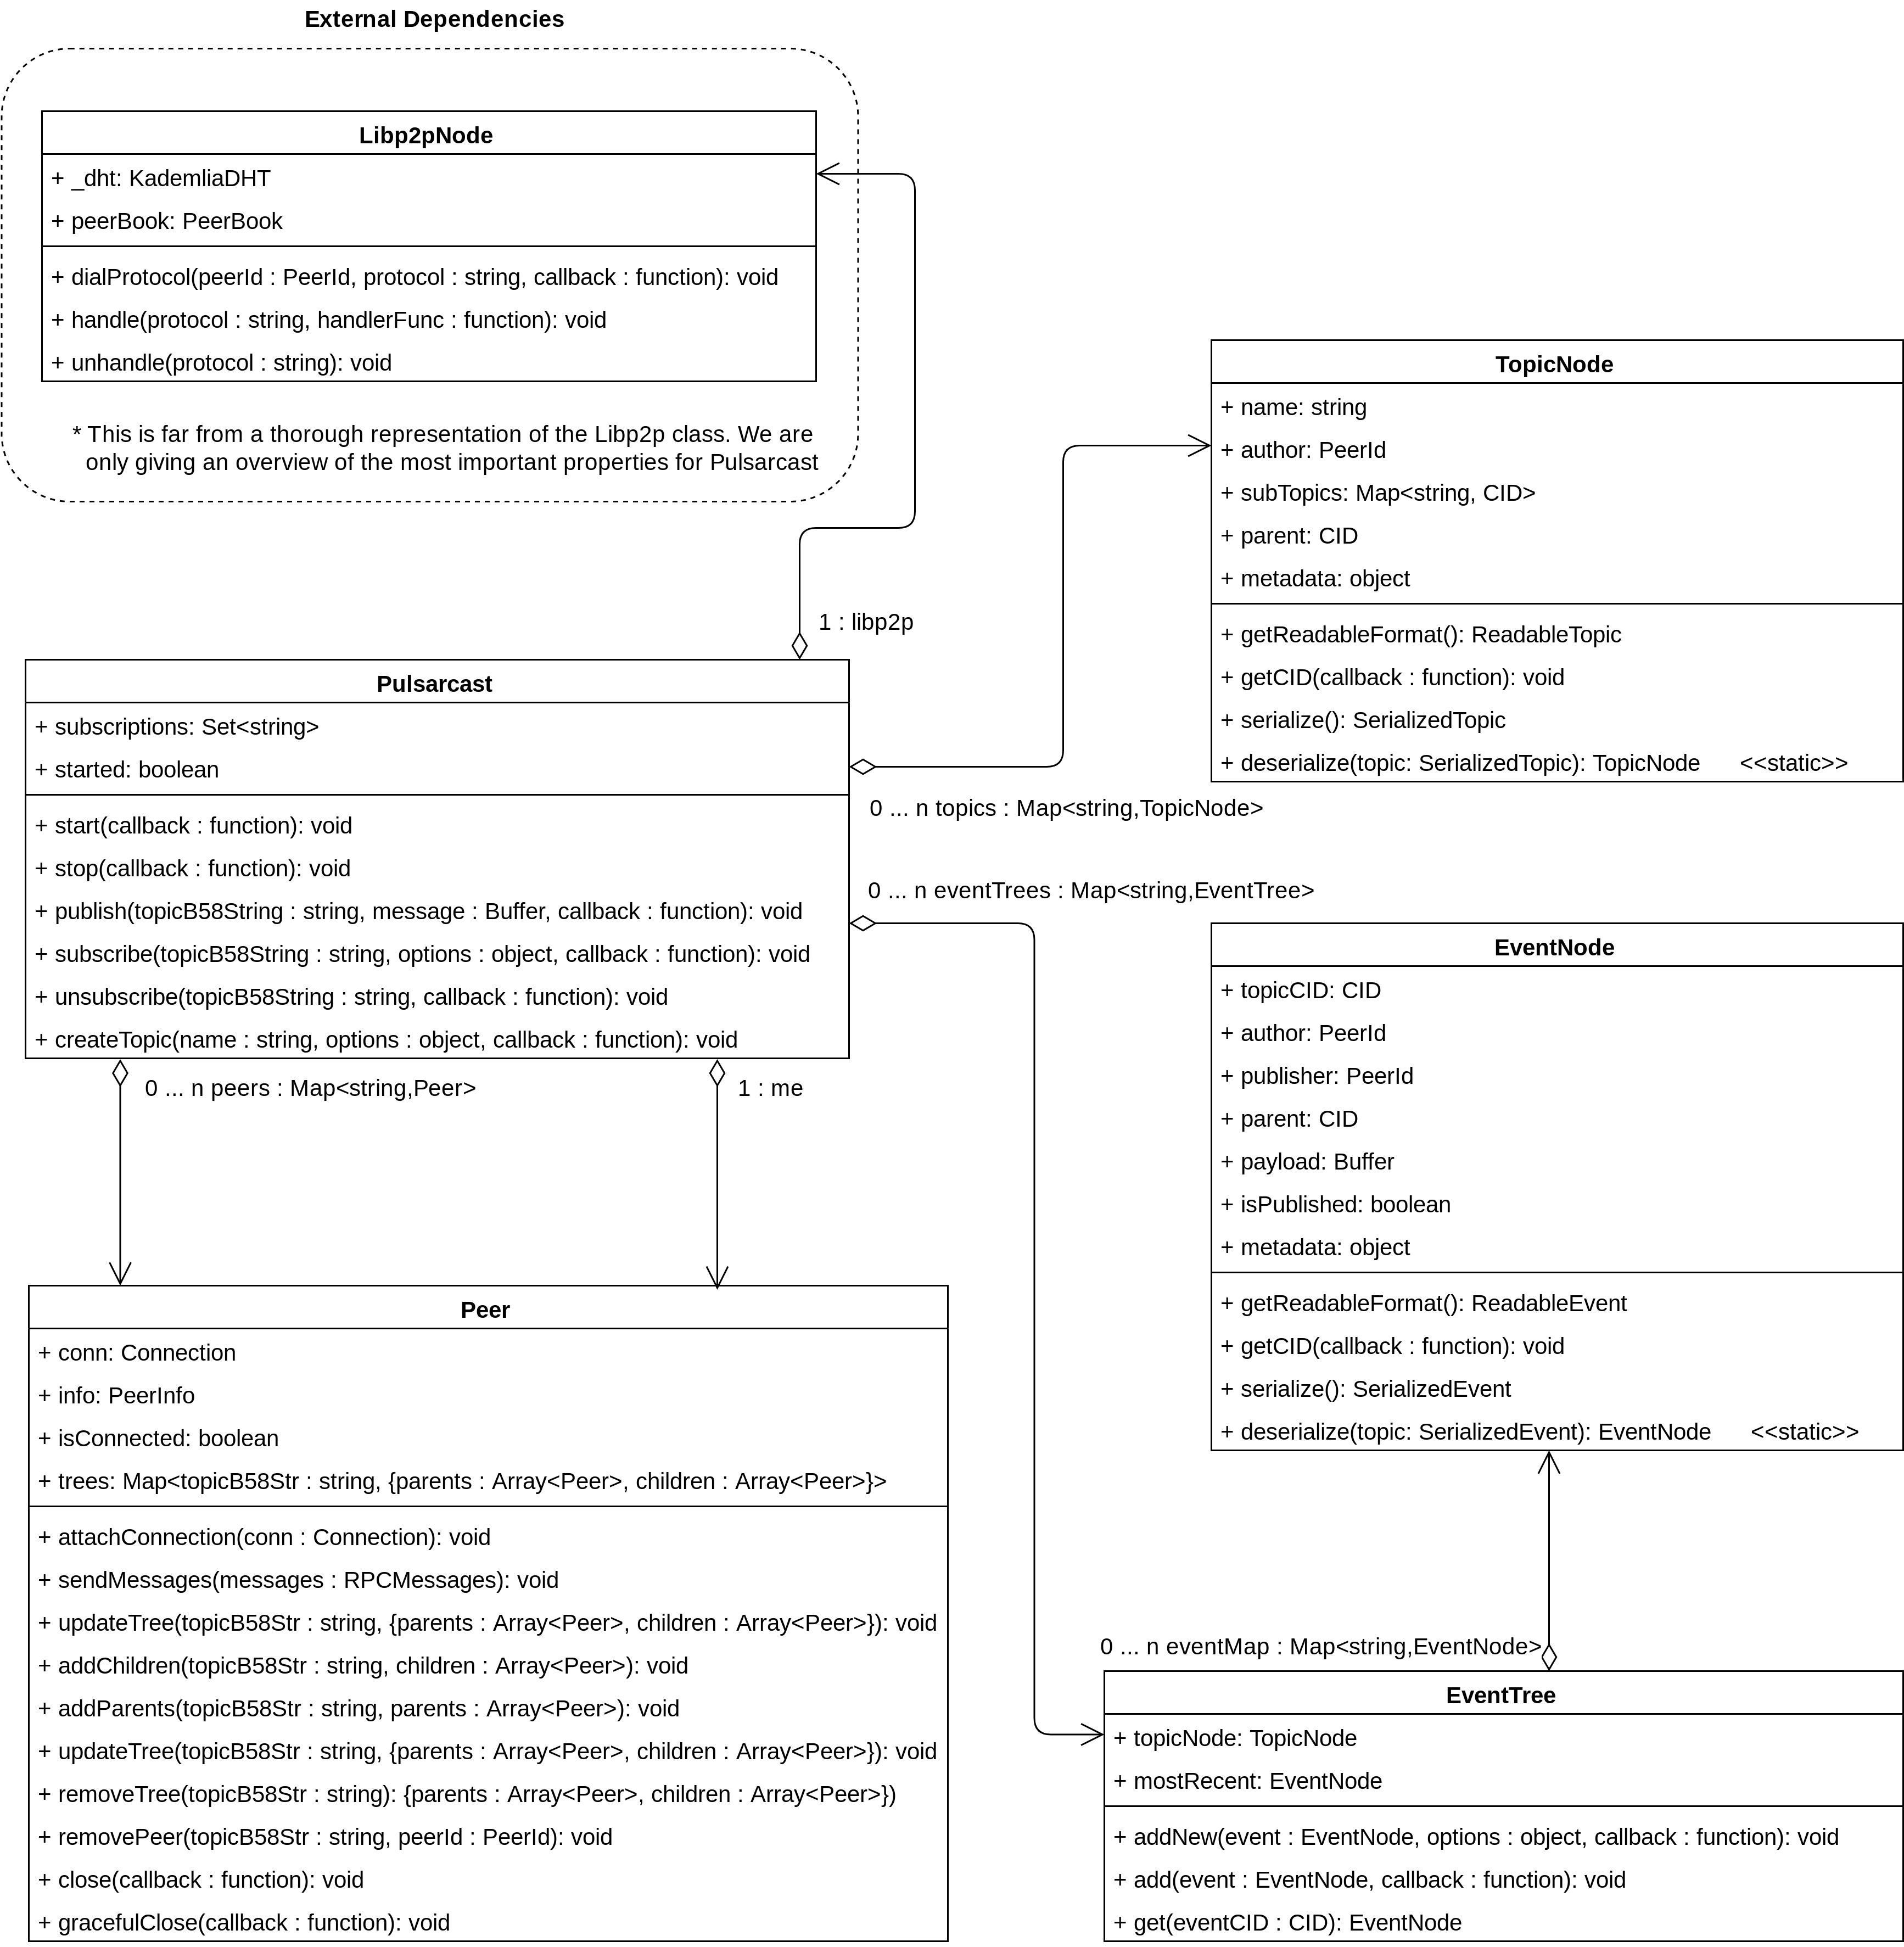
\includegraphics[width=1\textwidth]{img/uml-pulsarcast.png}
  \caption{\acrshort{uml} representation of the classes in our Pulsarcast system}
  \label{fig:pulsarcast-uml}
\end{figure}

\subsubsection{Pulsarcast}\label{subsubsec:pulsarcast}

Pulsarcast is our main class and essentially what makes a Pulsarcast node. It
contains the state of subscriptions, topics, connections and event
dissemination trees relevant to this node as well as the needed methods to
interact with the Pulsarcast underlying system. It extends the built-in
\verb|EventEmitter| class~\footnote{\url{https://nodejs.org/api/events.html}},
making our class capable of reproducing the event emitter
pattern~\footnote{\url{https://nodejs.dev/the-nodejs-event-emitter}}, the
mechanism we use to bubble up new Pulsarcast events to the application level.
It has a fairly simple constructor as one can see in Listing
\ref{pulsarcast-constructor}. The class has seven key methods exposed:

\begin{itemize}
  \item
    \verb|start(callback)| -  Start the Pulsarcast node by registering our protocol with the \emph{libp2p} protocol connection handler.
  \item
    \verb|stop(callback)| - Stop the Pulsarcast node, gracefully close connections we might have to any peer and de-register our protocol from the \emph{libp2p} protocol connection handler.
  \item
  \verb|createTopic(topicName, [options], callback)| - Create a Pulsarcast topic with the specified name. An optional object can be provided through which we can add \verb|subTopics|, \verb|parent| link and topic metadata configuration with \verb|allowedPublishers|, \verb|requestToPublish| and \verb|eventLinking|. By default, no \verb|parent| link is added and only the topic author is allowed to publish (essentially creating an event dissemination tree with order guarantee).
  \item
    \verb|subscribe(topicB58Str, [options], callback)| - Subscribe to a topic with the given base58 \acrshort{cid}. An option \verb|subscribeToMeta| can be provided which will determine if this node will subscribe to this topic's meta-topic also (defaults to true).
  \item
    \verb|unsubscribe(topicB58Str, callback)| - Unsubscribe from the topic with the given base58 \acrshort{cid}. An option \verb|unsubscribeFromMeta| can be provided which will determine if this node will unsubscribe to this topic's meta-topic also (defaults to true).
  \item
    \verb|publish(topicB58Str, message, callback)| - Publish the provided message in the topic with the given base58 string as a \acrshort{cid}.
\end{itemize}

% \noindent\begin{minipage}{\textwidth}
% \vspace{8pt}
\begin{lstlisting}[language=JavaScript, float, caption={Pulsarcast constructor},label={pulsarcast-constructor}]

class Pulsarcast extends EventEmitter {

  /**
   * Create a new Pulsarcast node.
   *
   * @param {external:Libp2pNode} libp2p
   * @param {object} [options={}] - Pulsarcast options
   */
  constructor(libp2p, options = {}) {
    super()

    this.libp2p = libp2p
    this.started = false

    this.peers = new Map()
    this.topics = new Map()
    this.subscriptions = new Set()
    this.eventTrees = new Map()

    this.me = new Peer(libp2p.peerInfo)
    this._onConnection = this._onConnection.bind(this)

    // Create our handlers to receive and send RPC messages
    this.rpc = createRpcHandlers(this)
  }

  (...)

}
\end{lstlisting}
% \vspace{8pt}
% \end{minipage}

Pulscarcast's topic creation, subscribe/unsubscribe and publish methods are
relatively simple, given our separation of concerns. All of them consist of a
set of input sanity checks with control, in the end, being handover to our
\acrshort{rpc} handlers, responsible for storing any relevant information in
the \acrshort{dht} and forwarding/creating any \acrshort{rpc} request that we
might need. Listing \ref{pulsarcast-subscribe} shows us an example of the logic
above, the subscribe method. New subscription calls in Pulsarcast are done
using the topic's base58 \acrshort{cid}. The Pulscarcast node keeps all the
state relative to the topics we are subscribed. As such, before performing any
action, we always check to see if we are subscribed to the topic given. If all
the input checks are right, we hand over to our \acrshort{rpc} handlers to
create the appropriate \acrshort{rpc} messages and forward our request.

% \noindent\begin{minipage}{\textwidth}
% \vspace{8pt}
\begin{lstlisting}[language=JavaScript, float, caption={Pulsarcast class subscribe method},label={pulsarcast-subscribe}]
  subscribe(topicB58Str, options, callback) {
    assert(this.started, 'Pulsarcast is not started')
    if (!callback) {
      callback = options
      options = {}
    }
    const topicCID = new CID(topicB58Str)
    // By default subscribe to meta topic
    const defaultSubscribeOptions = {
      subscribeToMeta: true
    }
    const subscribeOptions = { ...defaultSubscribeOptions, ...options }
    if (this.subscriptions.has(topicB58Str)) {
      return this._getTopic(topicCID, (err, topicNode) => {
        callback(err, topicNode, topicCID)
      })
    }
    this.subscriptions.add(topicB58Str)
    this.rpc.receive.topic.join(
      this.me.info.id.toB58String(),
      topicCID,
      subscribeOptions,
      callback
    )
  }
\end{lstlisting}
% \vspace{8pt}
% \end{minipage}

Although not part of the public methods we have mentioned, one key part of the
Pulsarcast class is the actual management of peers and connections (outgoing
and incoming). When the Pulsarcast node is started via the \verb|start| method,
we register our protocol \verb|/pulsarcast/1.0.0| with the \emph{libp2p}
protocol handlers. When an incoming connection that matches our protocol
reaches our node, the Pulsarcast class is responsible for internally handling
it, creating the necessary Peer objects and registering the appropriate
connection handlers so that when/if the connection drops we clear all the
relevant state. The same goes for when the node needs to contact another peer.
If a connection needs to be established, it is up to the Pulsarcast class to do
it properly. Listing \ref{pulsarcast-connection-handlers} gives us a thorough
look into the connection handling methods.

% \noindent\begin{minipage}{\textwidth}
% \vspace{8pt}
\begin{lstlisting}[language=JavaScript, float=p, caption={Pulsarcast internal peer and connection handlers. These methods abstract the logic of connection handling to all the other parts of the Pulsarcast system.},label={pulsarcast-connection-handlers}]
  _getPeer(peerId, callback) {
    const idB58Str = peerId.toB58String()
    const peer = this.peers.get(idB58Str)
    // We already have the peer in our list
    if (peer) return setImmediate(callback, null, peer)
    // Let's dial to it
    this.libp2p.dialProtocol(peerId, protocol, (err, conn) => {
      if (err) return callback(err)
      const peerInfo = this.libp2p.peerBook.get(peerId)
      const peer = this._addPeer(peerInfo, conn)
      callback(null, peer)
    })
  }

  _onConnection(protocol, conn) {
    conn.getPeerInfo((err, peerInfo) => {
      if (err) {
        // Terminate the pull stream
        return pull(pull.empty(), conn)
      }
      this._addPeer(peerInfo, conn)
    })
  }

  _listenToPeerConn(idB58Str, conn, peer) {
    pull(
      conn,
      lp.decode(),
      pull.map(data => protobuffers.RPC.decode(data)),
      pull.drain(
        rpc => this._onRPC(idB58Str, rpc),
        err => this._onConnectionEnd(err, idB58Str, peer)
      )
    )
  }
\end{lstlisting}
% \vspace{8pt}
% \end{minipage}

\subsubsection{Peer}\label{subsubsec:peer}

The Peer class provides an abstraction for the state of each peer, including
connections, information such its \acrshort{id} and address and the
dissemination trees it is part of. Listing \ref{peer-constructor} shows us the
constructor of our class. Its \verb|trees| property is a \verb|Map| indexed by
topic identifier, that keeps the peer's current dissemination trees neighbours.

\begin{lstlisting}[language=JavaScript, float=p, caption={Peer class constructor},label={peer-constructor}]
class Peer extends EventEmitter {
  constructor(peerInfo, conn = null) {
    log.trace('New peer registered %j', { peer: peerInfo.id.toB58String() })
    assert(peerInfo, 'Need a peerInfo object to initiate the peer')
    super()

    this.stream = null
    this.conn = conn
    this.info = peerInfo
    this.trees = new Map()

    if (conn) {
      this.attachConnection(conn)
    }
  }
  (...)
}
\end{lstlisting}

\subsubsection{TopicNode and EventNode}\label{subsubsec:topic-node}

The \verb|TopicNode| and \verb|EventNode| classes refer to our topic and event
descriptor dag nodes respectively. They are quite similar given that, in the
end, they both abstract Merkle \acrshort{dag} nodes. Listings \ref{topic-node-constructor}
and \ref{event-node-constructor} show us its constructors. Despite the
similarities, though, some aspects are worth noting. Such example is the
\verb|isPublished| field on the event descriptor. Which is crucial for our
system to understand if this event has or has not been published yet.

\begin{lstlisting}[language=JavaScript, float=p, caption={TopicNode class constructor},label={topic-node-constructor}]
class TopicNode {
  constructor(name, author, options = {}) {
    assert(author, 'Need an author to create a topic node')
    this.name = name
    this.author = author
    this.subTopics = {}
    this.parent = options.parent ? new CID(options.parent) : null
    if (options.subTopics) {
      this.subTopics = Object.entries(options.subTopics)
        .map(([name, topicB58Str]) => ({ [name]: new CID(topicB58Str) }))
        .reduce((topics, topic) => ({ ...topic, ...topics }), {})
    }
    this.metadata = createMetadata(options.metadata)
  }
  (...)
}
\end{lstlisting}

\begin{lstlisting}[language=JavaScript, float=p, caption={EventNode class constructor},label={event-node-constructor}]
class EventNode {
  constructor(topicCID, author, payload, options = {}) {
    assert(topicCID, 'Need a topicCID object to create an event node')
    assert(author, 'Need an author to create an event node')
    assert(payload, 'Need a payload to create an event node')
    this.topicCID = topicCID ? new CID(topicCID) : null
    this.author = author
    this.payload = payload
    this.publisher = options.publisher
    this.parent = options.parent ? new CID(options.parent) : null
    this.metadata = createMetadata(options.metadata)
  }

  get isPublished() {
    return Boolean(this.publisher)
  }
  (...)
}
\end{lstlisting}

Both of the classes have a series of methods which we consider worth describing:

\begin{itemize}
  \item
    \verb|getCID(callback)| - Given our descriptors are content-addressable, their identifiers are ever-changing depending on the values of their properties. This method returns, through the callback function, the \acrshort{cid} for this descriptor.
  \item
    \verb|getReadableFormat()| - Return an object whose properties are human-readable representations of the values of this object in the canonical format described in Chapter \ref{chapter:pulsarcast}. It consists mostly of returning all the \acrshort{cid}s as base 58 strings.
  \item
    \verb|serialize()| - Return an object in the canonical format described in Chapter \ref{chapter:pulsarcast} of the descriptor in question, with all the \acrshort{cid}s in binary format (buffers). Mostly useful for when we are about to convert this descriptor to a protocol buffer and forward it.
  \item
    \verb|deserialize(node)| - Convert a descriptor in a serialized format to an instance of its class, returning that same instance. A static method for each class.
\end{itemize}


\subsection{\acrshort{rpc} Handlers}\label{subsec:rpc-handlers}

Pulsarcast's \acrshort{rpc} handlers are responsible for containing the
implementation of the critical algorithms mentioned in Chapter
\ref{chapter:pulsarcast}. These functions are not only used by the Pulsarcast
class when a new command is invoked but are also registered to handle incoming
messages from other nodes.  A generic handler is responsible for receiving
every incoming message and, depending on the type of operation (see
\ref{proto-rpc-message}), forward it to the correct handler.

It is also the generic handler responsibility to validate incoming and outgoing
messages, making sure they obey our pre-defined schemas. This is important
because specific requirements and rules cannot be enforced at the protocol
buffer level. For this purpose, we use the already mentioned validation
library, Joi. Joi allows us to write up validation schemas that are easy to
cope with, in Javascript. Listing \ref{joi-schema-event-descriptor} provides an
example of such schema in practice.

\begin{lstlisting}[language=JavaScript, float=h, caption={Joi schema for and event descriptor},label={joi-schema-event-descriptor}]
const metadata = Joi.object()
  .keys({
    created: Joi.date().iso().required(),
    protocolVersion: Joi.string().required()
  }).required()

const eventDescriptor = Joi.object().keys({
  publisher: Joi.binary().required().allow(null),
  author: Joi.binary().required(),
  parent: Joi.object()
    .keys({
      '/': Joi.binary().allow(null)
    }).required(),
  payload: Joi.binary().required(),
  topic: Joi.object()
    .keys({
      '/': Joi.binary().required()
    }).required(),
  metadata
})
\end{lstlisting}

We have split our \acrshort{rpc} handlers into outgoing and incoming and tried
to reuse as much logic as possible. Hence why when the client invokes a new
command through the Pulsarcat \acrshort{api}, control is handed over to the
respective \acrshort{rpc} handler as if we had just received an \acrshort{rpc}
message from another node. Consequently, some of the logic described in the
algorithms in Chapter \ref{chapter:pulsarcast} is split between
incoming/outgoing \acrshort{rpc} handlers. The following list provides an
overview of the functions we have created:

\begin{itemize}
  \item
    \verb|rpc.receive.genericHandler()| - The generic handle responsible for receiving all the incoming \acrshort{rpc} messages, validating these and forwarding it accordingly.
  \item
    \verb|rpc.receive.publish()| - The receiving \acrshort{rpc} handler for publish events, responsible for partially implementing Algorithm \ref{alg:receive-event}. Upon receiving the \verb|eventNode| and the id of the peer sending it (\verb|idB58Str|), it starts by checking if the publish originated in that same node. Checks for the existence of the topic descriptor the event refers to and checks this node's permission to publish. Depending on the result, the function hands control over to the \verb|rpc.send.publish| function or \verb|rpc.receive.requestToPublish|. 
  \item
    \verb|rpc.receive.requestToPublish()| - The receiving \acrshort{rpc} handler for request to publish events, responsible for partially implementing Algorithm \ref{alg:receive-event}. Upon receiving the \verb|eventNode| and the id of the peer sending it (\verb|idB58Str|) checks for the existence of the topic descriptor the event refers to and checks this node's permission to request to publish. It then checks this node's permission to publish the event. Depending on the result, the function hands control over to the \verb|rpc.send.publish| function or the \verb|rpc.send.requestToPublish|. 
  \item
    \verb|rpc.receive.join()| - The receiving \acrshort{rpc} handler for a new subscription, responsible for partially implementing Algorithm \ref{alg:subscribe}. Upon receiving the \verb|topicCID| and the \acrshort{id} of the peer sending, it (\verb|idB58Str|) checks for the existence of the topic descriptor we want to join to and if the join command originated at this node. If not, it means we have received this join request from another node, as such, we need to add it to our event dissemination tree for this topic. With the new state appropriately set, we check if we are already part of this dissemination tree, if not we need to generate a join request ourselves and forward it, handing over control to \verb|rpc.send.publish|. 
  \item
    \verb|rpc.receive.leave()| - The receiving \acrshort{rpc} handler for unscribe requests. This function is similar to its counterpart responsible for subscribing to a topic.
  \item
    \verb|rpc.send.publish()| - The outgoing \acrshort{rpc} handler for event publishing, responsible for partially implementing Algorithm \ref{alg:send-event}. It starts by checking if the event is being created at this node. If it is, it links it to its parent event accordingly and stores it in the \acrshort{dht}. If the node is subscribed to this topic, the event is emitted to the application level. Finally, the event is forwarded to the branches of the dissemination tree who have not received it yet.
  \item
    \verb|rpc.send.requestToPublish()| - The outgoing \acrshort{rpc} handler for request to publish events, responsible for partially implementing Algorithm \ref{alg:send-event}, mainly consisting of forwarding the requests to the appropriate dissemination tree branches.
  \item
    \verb|rpc.send.join()| - The outgoing \acrshort{rpc} handler for subscription requests, responsible for partially implementing Algorithm \ref{alg:subscribe}. Upon being called, it looks up for the closest known peer to the topic author, locally stored in \acrshort{dht}. With the closest peer id, we update our node's dissemination tree parent for this topic and send our join \acrshort{rpc} request.
  \item
    \verb|rpc.send.leave()| - The outgoing \acrshort{rpc} handler for unsubscribe requests. Mostly the same logic as its counterpart \verb|join| but for leaving a topic.
  \item
    \verb|rpc.send.newTopic()| - This function handles the topic creation logic, responsible for implementing the Algorithm \ref{alg:new-topic}.  When called, it starts by validating the new topic, checking if its sub-topics and parent are valid and exist, creating a meta topic if one has not been provided already, storing these in the \acrshort{dht} and finally propagating the new topic through the meta-topic.
\end{itemize}

\subsection{Usage}\label{subsec:usage}

Listing \ref{pulsarcast-usage-example} provides a usage example of our
Javascript module. Keep in mind that this is a oversimplified example of
course, with a single node, its purpose is to understand how the \acrshort{api} comes
together and allows applications to integrate with it.

\begin{lstlisting}[language=JavaScript, float=h, caption={Usage example of our Pulsarcast module},label={pulsarcast-usage-example}]
const Pulsarcast = require('pulsarcast')

// node is a libp2p Node
const pulsarcastNode = new Pulsarcast(node)

const pulsarcastNode.start((err) => {
  if (err) console.log('No!!!', err)
  
  pulsarcastNode.createTopic('fuuuuun', (err, cid, topicNode) => {
    if (err) console.log('No!!!', err)
    console.log('Our new topic \o/', topicNode)
    
    pulsarcastNode.on(cid.toBaseEncodedString(), (eventNode) => {
      console.log('event', eventNode)
    })
    
    pulsarcastNode.publish(cid.toBaseEncodedString(), new Buffer('super fun!'), (err, eventCID) => {
      if (err) console.log('No!!!', err)
      console.log('published', eventCID.toBaseEncodedString())
    })
  })
})
\end{lstlisting}

\section{Testbed}\label{sec:testbed}

As part of our implementation, we needed a way to test our Pulsarcast system.
However we had a set of specific requirements that made our choice of tools
harder. We needed something that fulfilled the following:

\begin{itemize}
  \item Easily deploy and test different versions of our module.
  \item Run tests not only on Pulsarcast but also on \acrshort{ipfs}' own pub-sub
    implementation.
  \item Able to extract relevant usage metrics.
  \item Simulate network constraints such as latency.
  \item Able to run locally but easily scalable to a large network.
  \item Can be controlled from a central point, while being able to interact
    with specific nodes in the system.
  \item Easy to create scripts for, so that we could automate as much of our
    test suite as possible.
\end{itemize}

Unfortunately for us, we could not find a tool that, straight out of the box,
ticked all of these requirements. We were then faced with the need to create
our own testbed which we further detail in the next sections.

\subsection{Architecture}\label{subsec:testbed-architecture}

If we look carefully into the set of
requirements above we see that a core principle that can be extracted is
reproducibility. Reproducibility allows us to run our testbed locally or in a
cloud service somewhere in the world and still expect the same behaviour and
results. Reproducibility is usually achieved through virtualisation mechanisms
that allow a certain workload to behave and act the same, whether we are
running it locally in our workstation or in a machine with different
specifications in the other end of the world. Nowadays this is most commonly
done through containerisation
techniques~\footnote{\url{https://www.freebsd.org/doc/handbook/jails.html}}~\footnote{\url{https://blog.jessfraz.com/post/containers-zones-jails-vms}}
with tools such as
Docker~\footnote{\url{https://www.docker.com/products/container-runtime}}, which we
used to create a containerised version of our module. To orchestrate our
containerised application we used Kubernetes~\footnote{\url{https://kubernetes.io/}},
an open source orchestration platform based on Google's learnings on running
containerised workloads at
scale~\footnote{\url{https://research.google/pubs/pub43438/}}, and one of the most
popular solutions in the field.

Kubernetes exposes a set of relevant usage
metrics~\footnote{\url{https://kubernetes.io/docs/tasks/debug-application-cluster/resource-metrics-pipeline/}}~\footnote{\url{https://github.com/kubernetes/kube-state-metrics}}
however we still need to process, aggregate and correlate these with the data
from our test runs. In order to do this we rely on
Elasticsearch~\footnote{\url{https://www.elastic.co/products/elasticsearch}} to store
metrics and test result data. Prior to consumption by the Elasticsearch, the
data is piped through
Logstash~\footnote{\url{https://www.elastic.co/products/logstash}} for adequate
processing. At each Kubernetes node, a couple of agents entitled
Beats~\footnote{\url{https://www.elastic.co/products/beats}} are responsible for
forwarding metrics and test data acquired through logs (events published,
messages sent, etc.). The final piece of the puzzle is
Kibana~\footnote{\url{https://www.elastic.co/products/kibana}}, used to query data
and build useful visualisations. Together, all these tools are commonly
referred to as the Elastic
Stack~\footnote{\url{https://www.elastic.co/products/elastic-stack}} and are the key
to how we gather results from our test runs. Figure
\ref{fig:ipfs-testbed-and-metrics} provides an overview of this pipeline in
practice.

As we know it, Pulsarcast is just a module that applications can use to build
on top of. In order to test it properly we needed something to allow us to
perform operations on demand in a Pulsarcast network (create a topic, subscribe
publish, etc.). For both simplicity sake but also because we wanted to use it
as our own test baseline, we've created a fork of the Javascript
\acrshort{ipfs} module, and some of its dependencies, that instantiates and
exposes a Pulsarcast node.  We stripped it down of anything that it didn't need
in order to run Pulsarcast and its own version of pub-sub, so that we could
avoid having extraneous logic disturb our test results and/or increase resource
consumption. This way we got an application which exposed an \acrshort{http}
\acrshort{api} that allowed us to interact with both systems (Pulsarcast and
\acrshort{ipfs}' pub-sub). The source code for this fork is available and open
source~\footnote{\url{https://github.com/jgantunes/js-ipfs}}.

In order to accurately test our solution we needed a way to simulate abnormal
network conditions. Toxiproxy~\footnote{\url{http://toxiproxy.io}} ended up being our
tool of choice. Toxiproxy worked by acting as a \acrshort{tcp} proxy that,
programmatically through an \acrshort{http} \acrshort{api}, allowed us to
inject multiple kinds of faults (known as toxics in the project). By putting it
in front of our \acrshort{ipfs} nodes we were able to simulate different
network conditions.  Figure \ref{fig:ipfs-testbed-and-metrics} provides a
visual explanation on how our \acrshort{ipfs} deployment and Toxiproxy fit
together.

\begin{figure}[!htb]
  \centering
  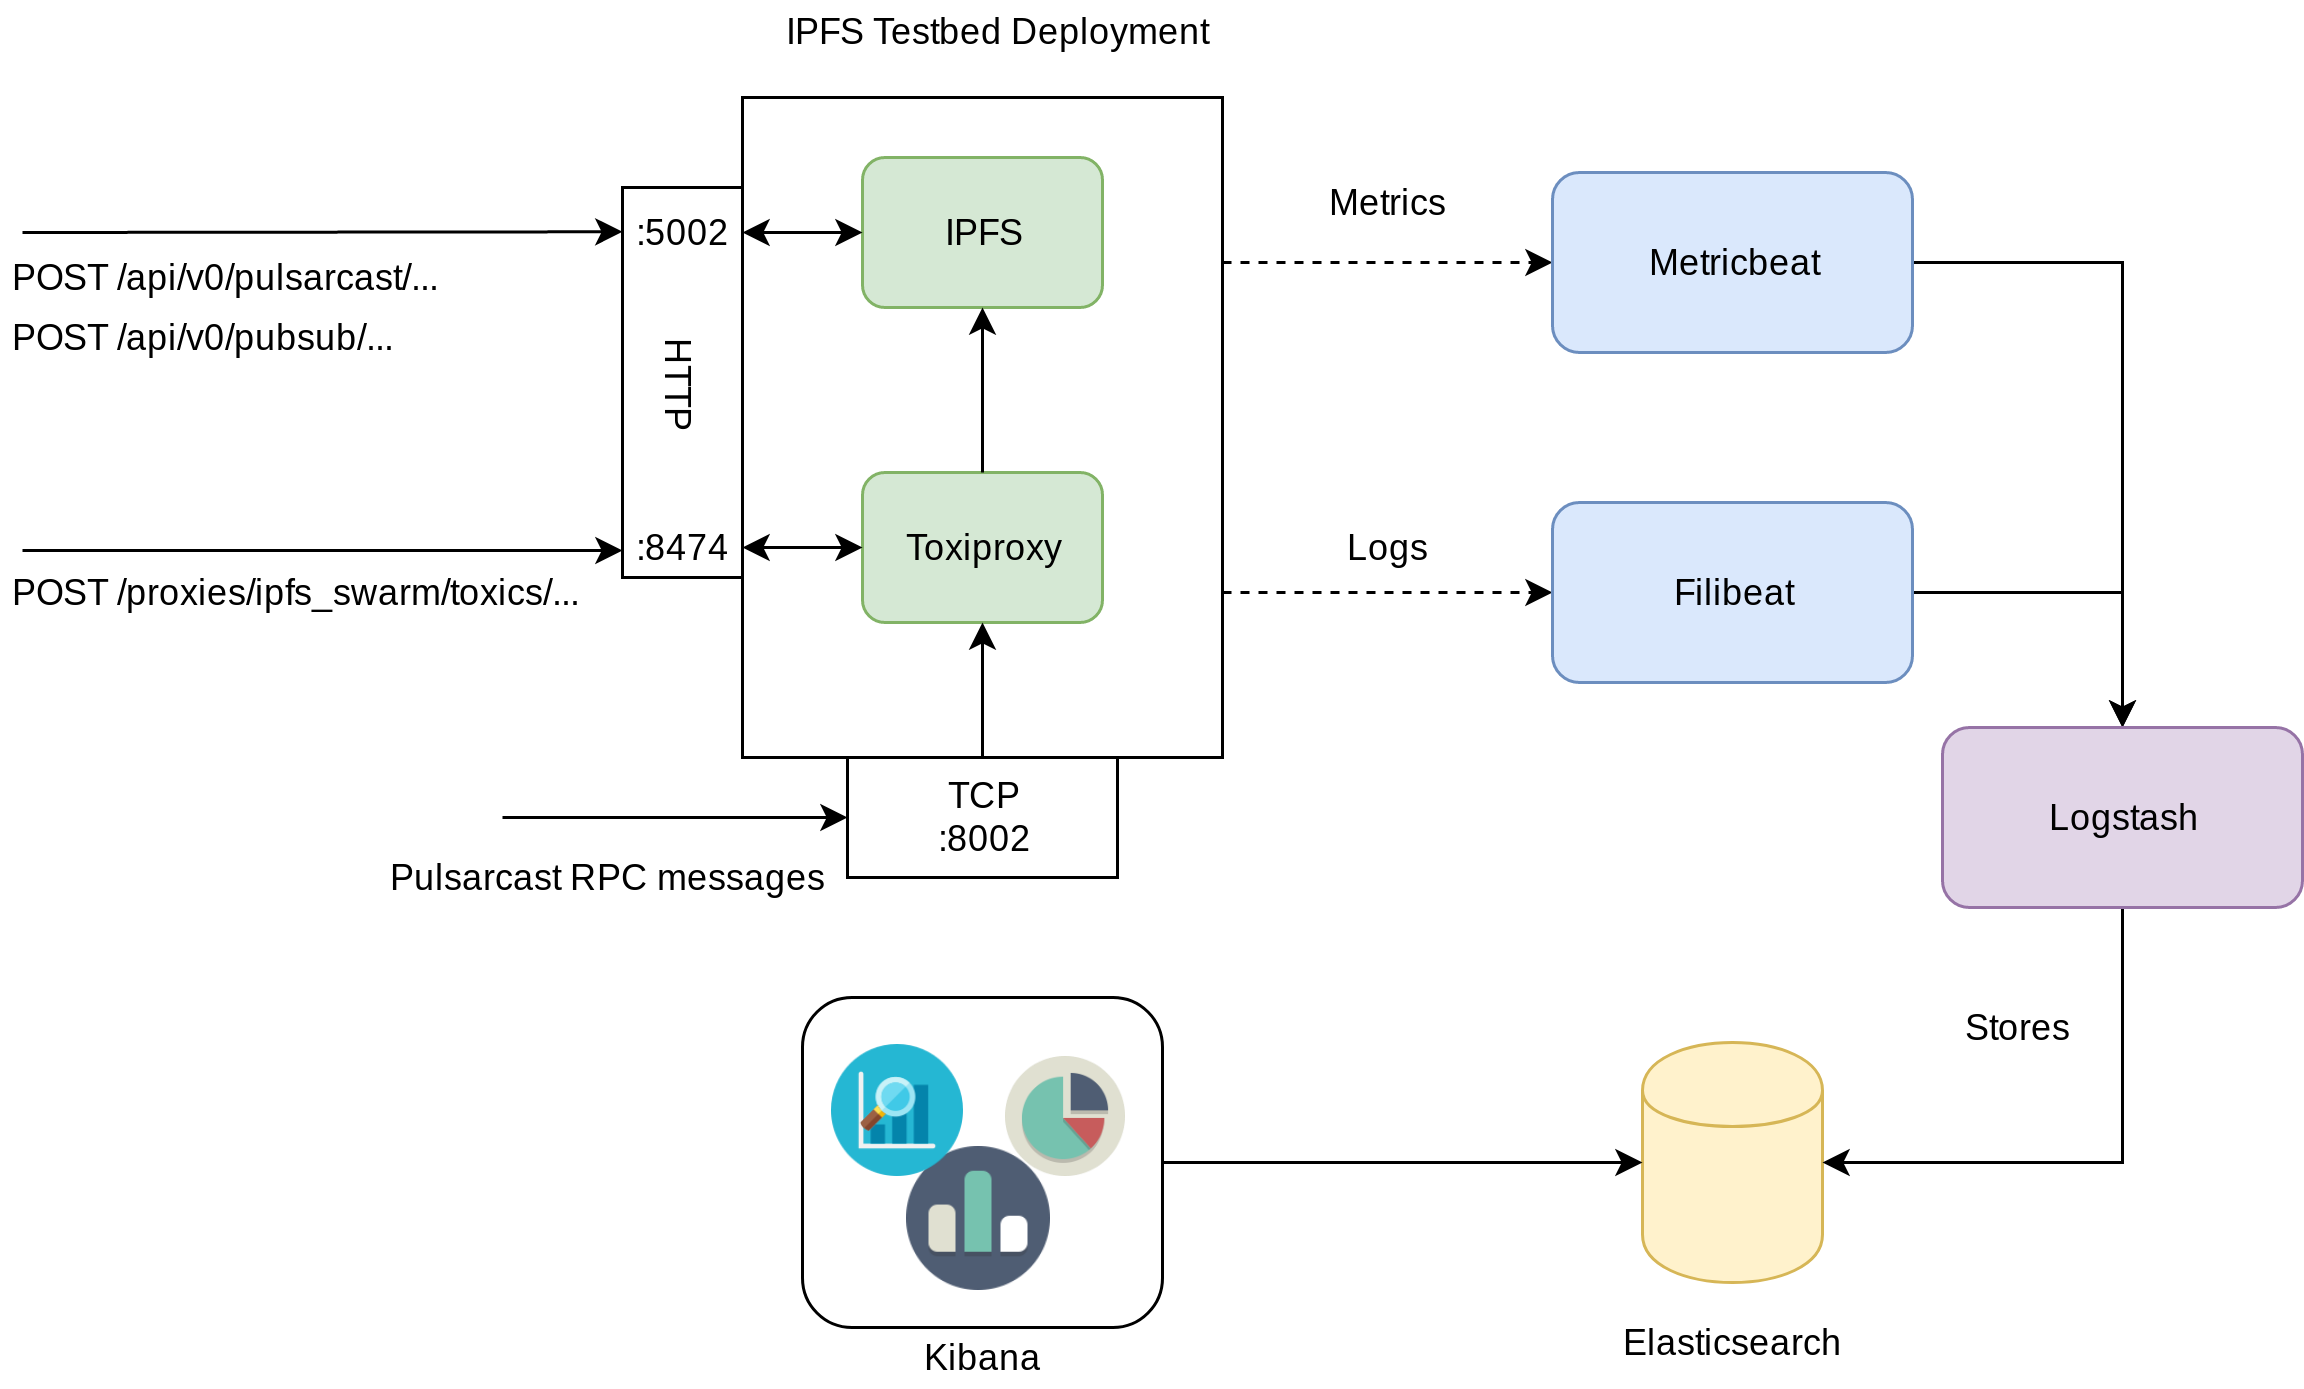
\includegraphics[width=0.95\textwidth]{img/ipfs-testbed-and-metrics.png}
  \caption{Overview of our ipfs-testbed deployment and our metrics/logs
  pipeline}
  \label{fig:ipfs-testbed-and-metrics}
\end{figure}

Our \acrshort{ipfs} deployment together with Toxiproxy makes up a configurable deployment
to which we call \acrshort{ipfs} Testbed. The template for this deployment (built using
Helm~\footnote{\url{https://helm.sh/}}) can be seen in our Helm Charts
repository~\footnote{\url{https://github.com/JGAntunes/helm-charts/tree/master/ipfs-testbed}}.

This whole setup has been coded so that we can run it in an automated fashion,
being able to bootstrap the Kubernetes cluster, deploy the Elastic Stack and
deploy any amount of \acrshort{ipfs} Testbed nodes. Figure
\ref{fig:ipfs-testbed-kubernetes-overview} gives us an idea of what this would
look like. As usual, the logic for this is open source and
accessible~\footnote{\url{https://github.com/JGAntunes/ipfs-testbed}}.

\begin{figure}[!htb]
  \centering
  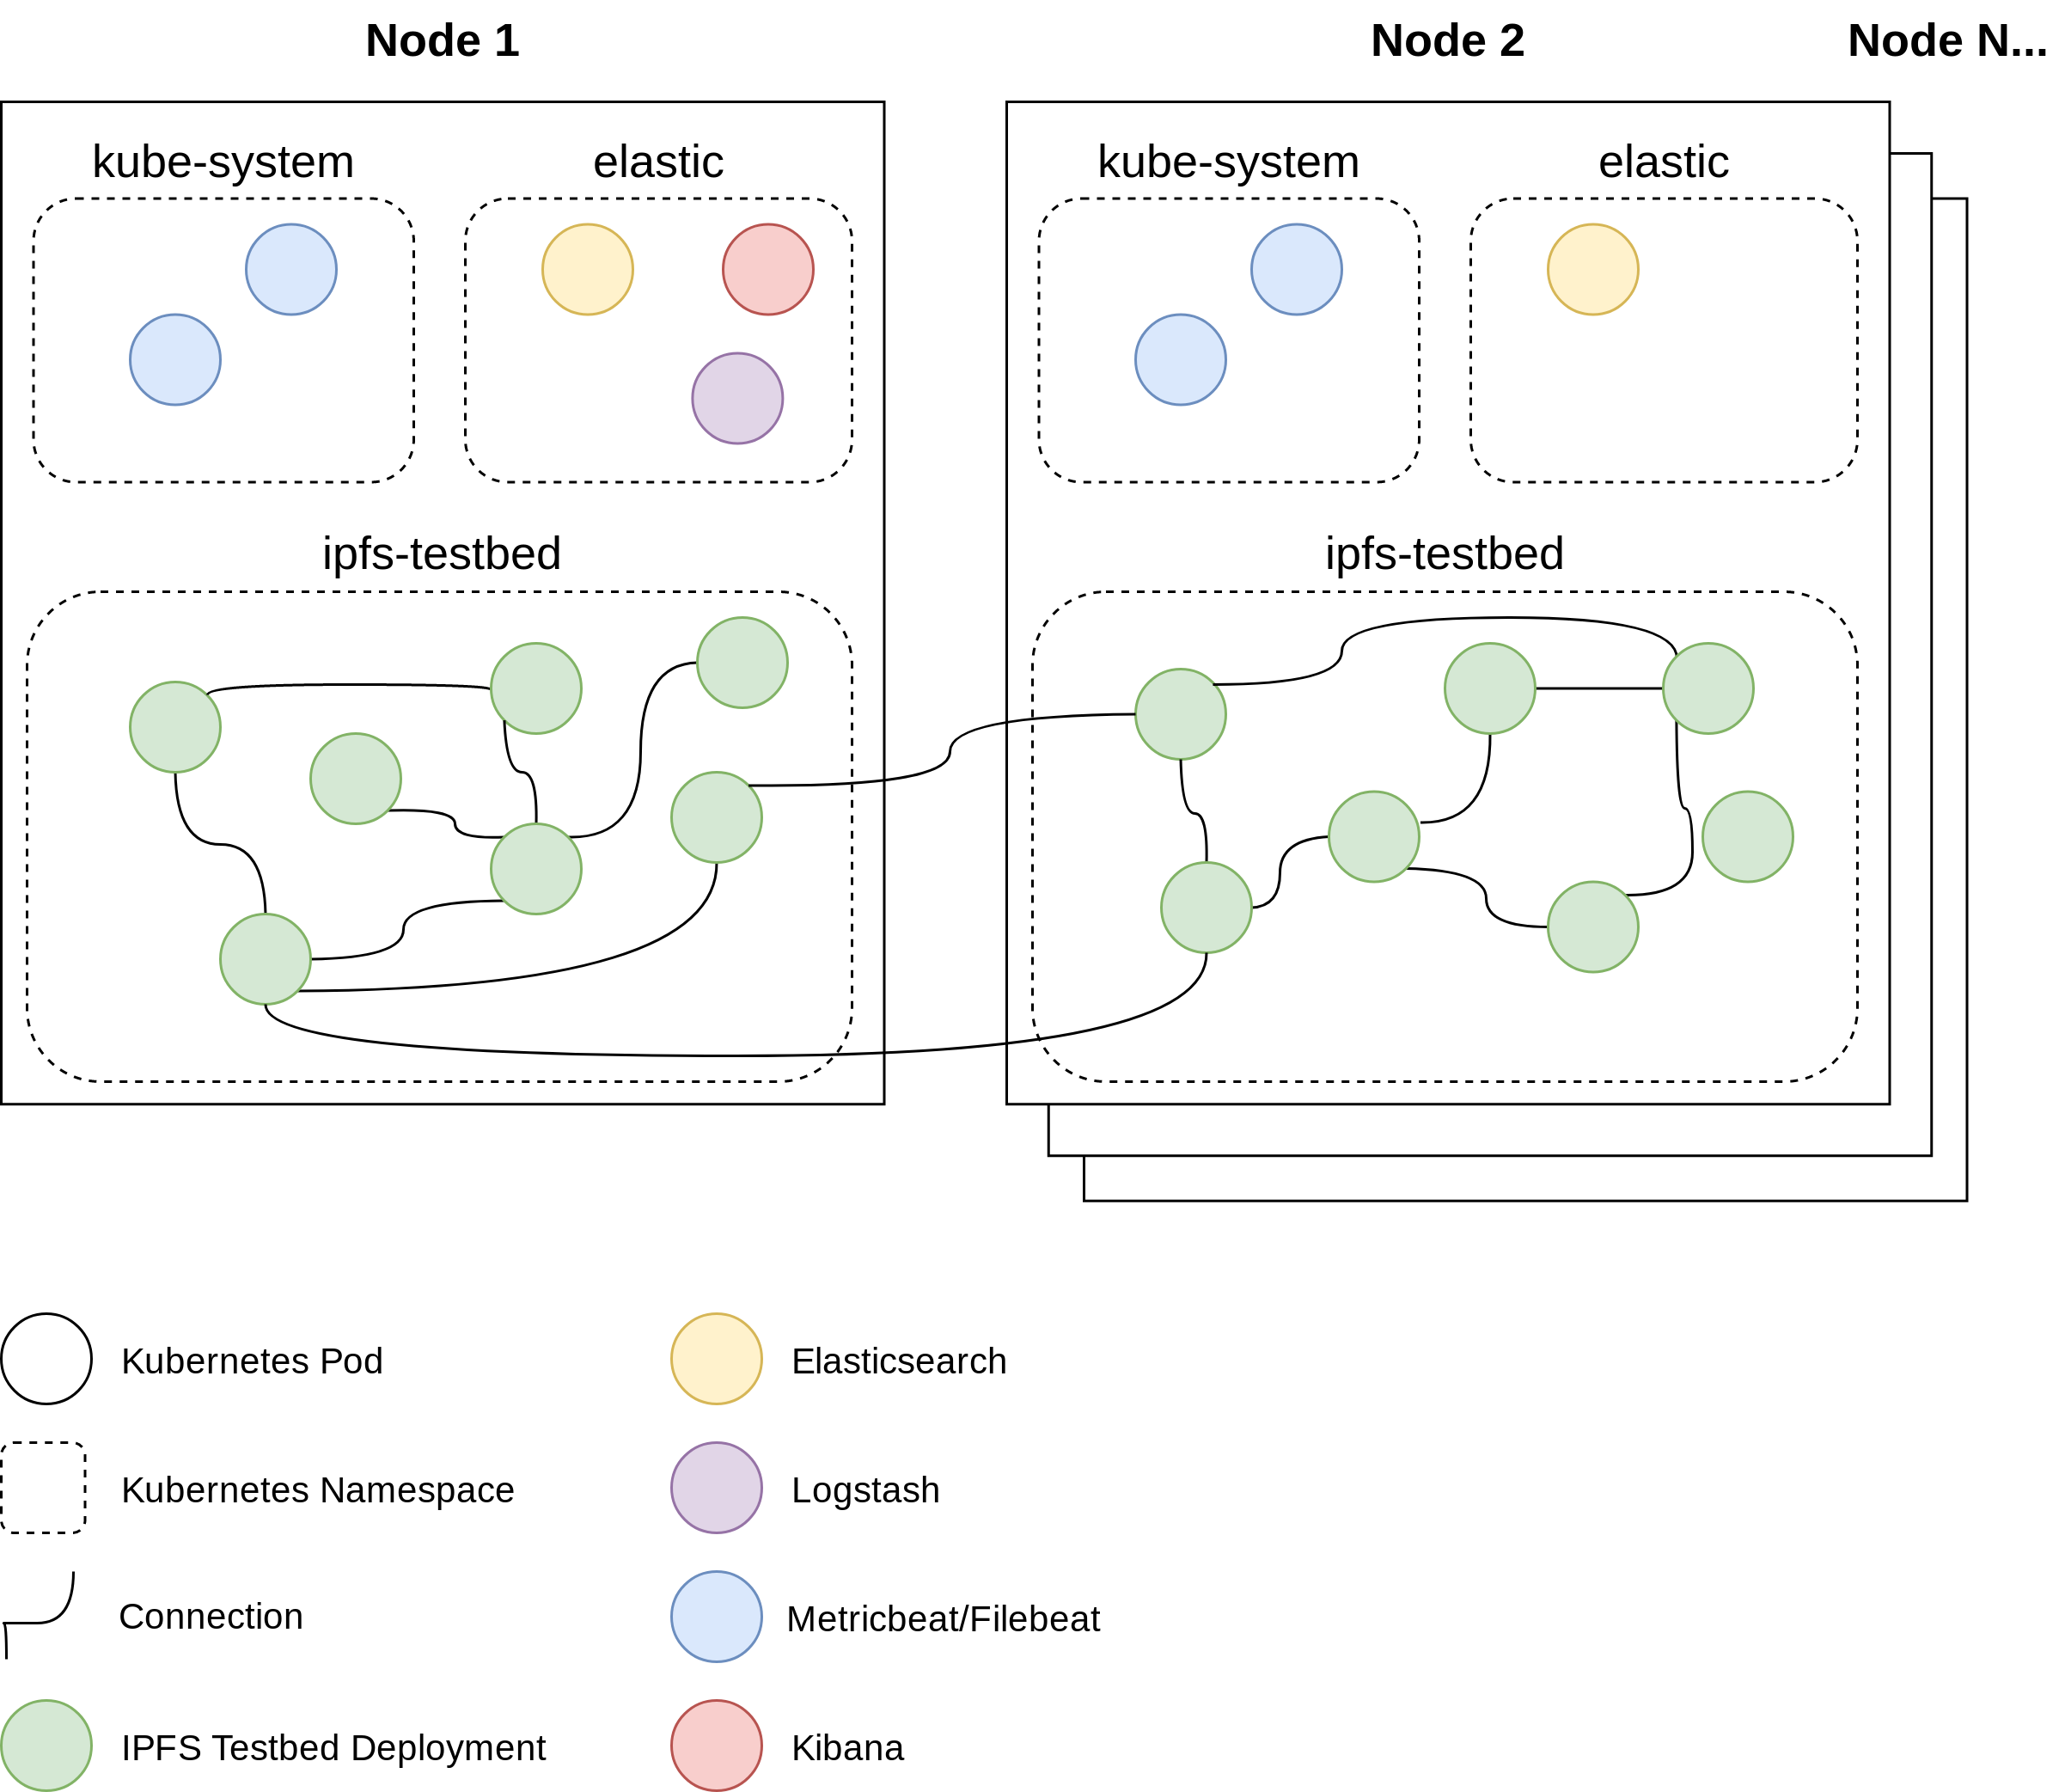
\includegraphics[width=0.95\textwidth]{img/ipfs-testbed-kubernetes-overview.png}
  \caption{Example of our system deployed in a Kubernetes cluster}
  \label{fig:ipfs-testbed-kubernetes-overview}
\end{figure}

\subsection{Usage}\label{subsec:testbed-usage}

After our testbed is built and running, we still need to come up with a way to
easily interact with it. Our goal was to able to orchestrate everything from a
single machine and, of course, make it in a way that can easily be automated so
that human intervention is barely required. For this purpose, we have built a
\acrshort{cli} tool that allows us to interact with our testbed nodes, named
ipfs-testbed-cli~\footnote{\url{https://github.com/JGAntunes/ipfs-testbed-cli}}. 

Under the hood our tool interacts with the Kubernetes \acrshort{api} Server,
using the credentials locally stored in the machine, to extract the addresses
for our testbed node's \acrshort{ipfs} and Toxiproxy \acrshort{api}s. Throw
these we can inject either \acrshort{ipfs} commands or Toxiproxy configurations
in any node. Listing \ref{ipfs-testbed-cli-examples} gives us a set of example
usages. Specifically, for our test runs, we have introduced two commands that
allowed for running a set of bulk operations using \acrshort{ipfs}' Floodsub
and Pulsarcast \acrshort{api}s.  Our Toxiproxy command also supported bulk
creation. This allowed us to automate most of our test executions to a couple
of one-line commands from our machine.

% \noindent\begin{minipage}{\textwidth}
% \vspace{8pt}
\begin{lstlisting}[language=bash, float, caption={\acrshort{ipfs} Testbed \acrshort{cli} example
usages},label={ipfs-testbed-cli-examples}]
# Create latency toxics of 500 ms with 300 ms jitter on all of the nodes (bulk=1)
 >$ ipt create toxic latency --latency=500 --jitter=300 --bulk=1

# Execute a ping from one node to another
 >$ ipt exec ping <from-peer-id> <to-peer-id>

# Execute a create pulsarcast topic command at node-1
 >$ ipt exec pulsarcast create sports --node-id=node-1

# Execute a floodsub subscribe command at node-1
 >$ ipt exec floodsub subscribe sports --node-id=node-1

# Execute a series of bulk pulsarcast commands from file
 >$ ipt exec pulsarcast load some-bulk-file

# Execute a series of bulk floodsub commands from file
 >$ ipt exec floodsub load some-bulk-file

\end{lstlisting}
% \vspace{8pt}
% \end{minipage}

\section{Summary}\label{summary}

Throughout this chapter, we covered the implementation of our Pulsacast
architecture and specification in Section \ref{pulsarcast-javascript-module}.
We started by briefly describing our Javascript module, its libp2p dependencies
and the way it fits together with the libp2p ecosystem. Afterwards, we
deep-dived into our module. Its code organisation, structure, as well as the
classes that constitute the backbone of it. Next in our list, we looked into
our \acrshort{rpc} handlers, responsible for implementing Pulsarcast's core
logic of subscription management and event dissemination.  Finally, we provided
a simple usage example of our module.

However, as we pointed out, we needed a way to test our system reliably. Given
we could not find anything that supported our requirements for flexibility of
deployment, control, and reproducibility, we had to build it ourselves. Section
\ref{sec:testbed} details our chosen solution. We created a reproducible
deployment of IPFS containing our Pulsarcast implementation with Toxiproxy
acting as an inbound \acrshort{tcp} proxy. This artefact is then deployed and
scaled as needed in a Kubernetes cluster, who collects metrics and logs using a
stack of Elasticsearch, Beats, Logstash and finally Kibana for visualisation.
